\noindent 2. \textbf{Circle} the script that makes the sprite do the same thing as the loop above: \\ \\
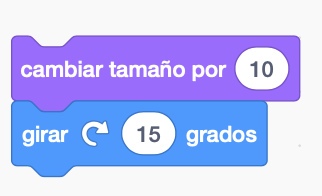
\includegraphics[scale=.3,valign=t]{q2_script1.png} \hspace{1.25cm}
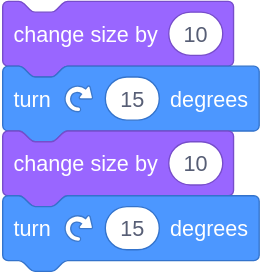
\includegraphics[scale=.3,valign=t]{q2_script2.png} \hspace{1.25cm}
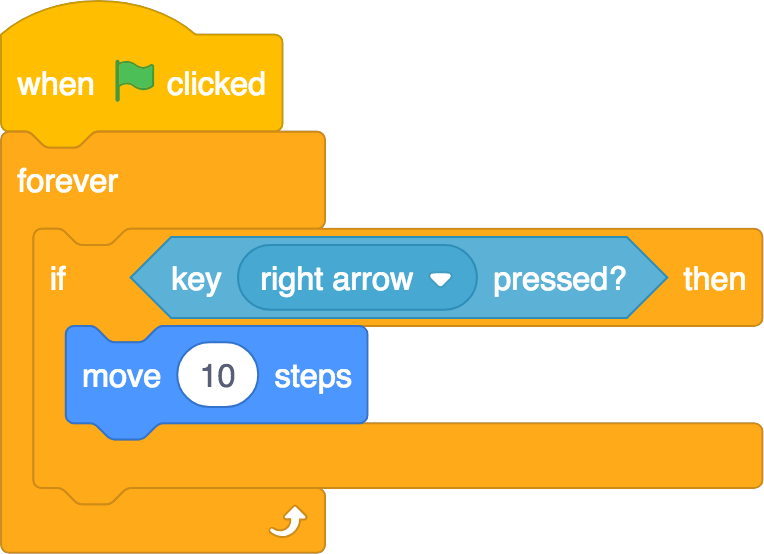
\includegraphics[scale=.3,valign=t]{q2_script3.png} \hspace{1.25cm}
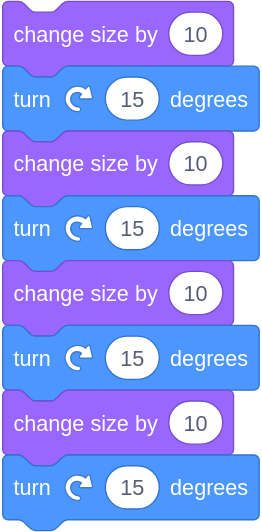
\includegraphics[scale=.3,valign=t]{q2_script4.png} \hspace{1.25cm} \\

\noindent \dotfill

\noindent 3. \textbf{Circle \underline{ALL}} the scripts that make the sprite change costumes \textbf{exactly} 3 times. \\

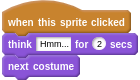
\includegraphics[scale=.3,valign=t]{q3_script0.png} \hspace{1.5cm}
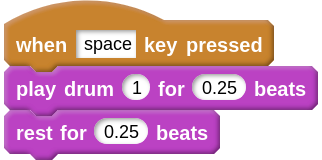
\includegraphics[scale=.3,valign=t]{q3_script1.png} \hspace{1.5cm}
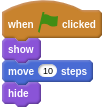
\includegraphics[scale=.3,valign=t]{q3_script2.png} \hspace{1.5cm}
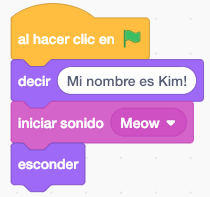
\includegraphics[scale=.3,valign=t]{q3_script3.png} \hspace{1.5cm} \\


\noindent \dotfill \\

\begin{center}
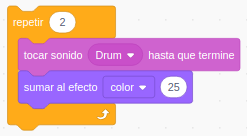
\includegraphics[scale=.3]{q4_script0.png}
\end{center}

\noindent 4. \textbf{Circle} the script that makes the sprite do the same thing as the loop above: \\ \\
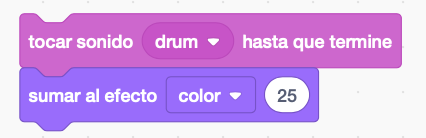
\includegraphics[scale=.25,valign=t]{q4_script1.png} \hspace{1.25cm}

\includegraphics[scale=.25,valign=t]{q4_script2.png} \hspace{1.25cm}
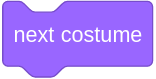
\includegraphics[scale=.25,valign=t]{q4_script3.png} \hspace{1.25cm}

\includegraphics[scale=.25,valign=t]{q4_script4.png} \hspace{1.25cm} \\

\noindent \dotfill \\

\begin{center}
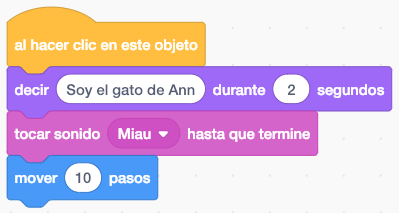
\includegraphics[scale=.3]{q5_script0.png}
\end{center}

\noindent 5a. \textbf{Circle \underline{ALL}} the blocks that run \underline{6 times} in the script above. \\ \\
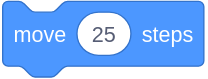
\includegraphics[scale=.3]{q5_script1.png} \hspace{1cm}
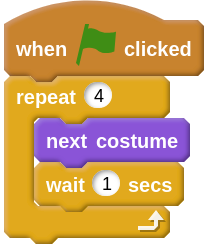
\includegraphics[scale=.3]{q5_script2.png} \hspace{1cm}
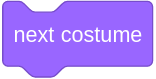
\includegraphics[scale=.3]{q5_script3.png} \hspace{1cm}
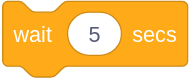
\includegraphics[scale=.3]{q5_script4.png} \hspace{1cm}\\

\noindent 5b. \textbf{Circle \underline{ALL}} the blocks that run \underline{before} the repeat loop in the script above. \\ \\
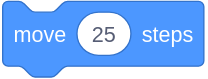
\includegraphics[scale=.3]{q5_script1.png} \hspace{1cm}
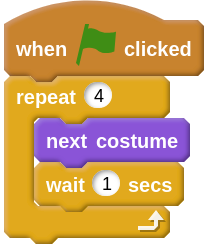
\includegraphics[scale=.3]{q5_script2.png} \hspace{1cm}
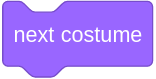
\includegraphics[scale=.3]{q5_script3.png} \hspace{1cm}
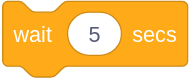
\includegraphics[scale=.3]{q5_script4.png} \hspace{1cm}\\

\noindent 5c. \textbf{Circle \underline{ALL}} the blocks that run \underline{after} the repeat loop in the script above. \\ \\
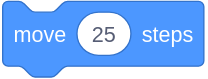
\includegraphics[scale=.3]{q5_script1.png} \hspace{1cm}
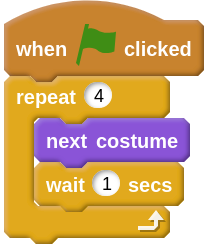
\includegraphics[scale=.3]{q5_script2.png} \hspace{1cm}
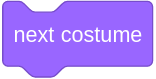
\includegraphics[scale=.3]{q5_script3.png} \hspace{1cm}
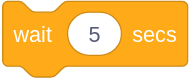
\includegraphics[scale=.3]{q5_script4.png} \hspace{1cm}\\

\noindent \dotfill \\

\newpage

\indent 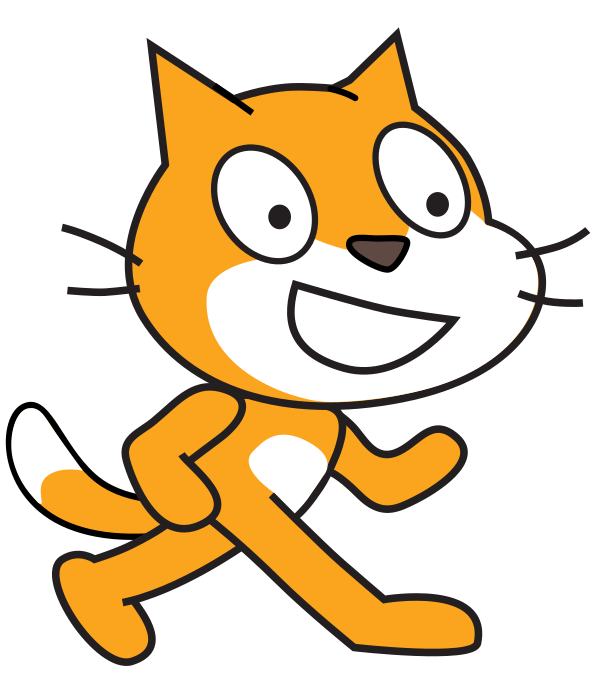
\includegraphics[scale=.25,valign=c]{cat.png} \underline{Cat's Code} \hspace{5cm}
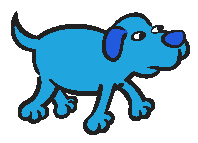
\includegraphics[scale=.2,valign=c]{dog.png} \underline{Dog's Code} \\
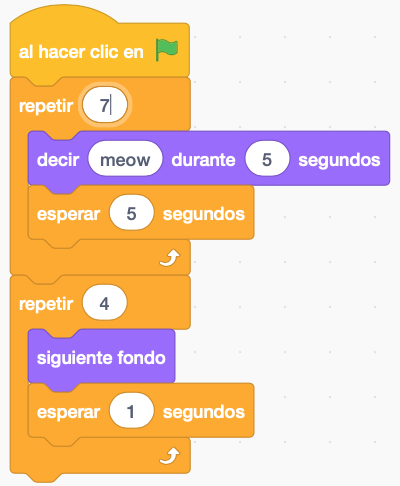
\includegraphics[scale=.3,valign=t]{q6_script0.png} \hspace{1cm}
 \vline height .75cm width 2pt \hspace{1cm}
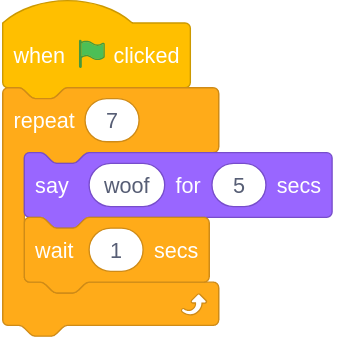
\includegraphics[scale=.3, valign=t]{q6_script1.png} \hspace{1cm}
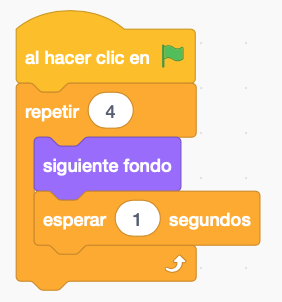
\includegraphics[scale=.3, valign=t]{q6_script2.png} \\ 

\noindent 6a. \textbf{Circle}: When the green flag is clicked, what will Cat do?
\renewcommand{\theenumi}{\Alph{enumi}}
\begin{enumerate}
\item Cat says "meow" 7 times \textbf{then} changes costumes 4 times.
\item Cat says "meow" and changes costumes \textbf{at the same time}. \\
\end{enumerate}

\noindent 6b. \textbf{Circle}: When the green flag is clicked, what will Dog do?
\renewcommand{\theenumi}{\Alph{enumi}}
\begin{enumerate}
\item Dog says "woof" 7 times \textbf{then} changes costumes 4 times.
\item Dog says "woof" and changes costumes \textbf{at the same time}.
\end{enumerate}

\noindent \dotfill \\
